\section{Opis aplikacji}
Aplikacja ma za zadanie umożliwienie użytkownikowi zbudowania diagramu PERT (Program Evaluation Review Technique) na który składają się kamienie milowe (milestone'y) oraz zadania (task) pomiędzy nimi.

Użytkownik może umieszczać poszczególne kamienie milowe na obszarze roboczym oraz tworzyć połączenia między nimi. Połączenia symbolizują zadania do wykonania. Istnieją dwa specjalne kamienie milowe: rozpoczęcie projektu oraz jego zakończenie.

Dla każdego z połączeń (zadań), użytkownik jest w stanie dodać opis oraz szacowany czas jego wykonania (optymistyczny, najbardziej prawdopodobny i pesymistyczny). 

Istnieje również możliwość dodawania ,,sztucznych'' aktywności (t.j. aktywności bez zadań, które pokazują jedynie zależności pomiędzy poszczególnymi kamieniami milowymi)

Na podstawie podanych czasów (oraz wszystkich zależności pomiedzy zadaniami) aplikacja dokonuje obliczeń kiedy każdy z kamieni milowych powinien być osiągnięty.

Aplikacja jest w stanie pokazać ścieżkę krytyczną w projekcie.

Aplikacja jest w stanie określić, czy utworzony diagram nie jest błędny (graf powinien być spójny i acykliczny, a każdy z jego wierzchołków powinien być połączony ścieżką do wierzchołka końcowego)

Istnieje możliwość wyeksportowania diagramu w formacie graficznym (np. SVG). Istnieje również możliwość eksportu diagramu do formatu JSON, który umożliwi późniejszą jego edycję.

Aplikacja zapewnia uwierzytelnianie i autoryzację użytkowników.

Zalogowany użytkownik ma możliwość zapisu diagramu na serwerze oraz późniejsze jego odczytanie.

Z przygotowanego diagramu PERT istnieje możliwość wygenerowania odpowiadającego mu diagramu Gantta.

Istnieje możliwość zapisu danej wersji diagramu i jego późniejsza aktualizacja, dzięki czemu jesteśmy w stanie nie tylko dokonywać adaptacji, ale również ocenić jakość naszych estymat w trakcie prowadzenia projektu.

Aplikacja powinna prawidłowo działać we wszystkich nowoczesnych przeglądarkach. Aplikacja jest rozwijana w technologii desktop-first - edycja diagramów na wyświetlaczach telefonów komórkowych nie jest rozważana.

Aplikacja może wspierać pracę na tablecie (zdarzenia dotykowe powinny być obsługiwane).

\subsection{Wygląd interfejsu użytkownika}
\begin{figure}[h]
	\centering
	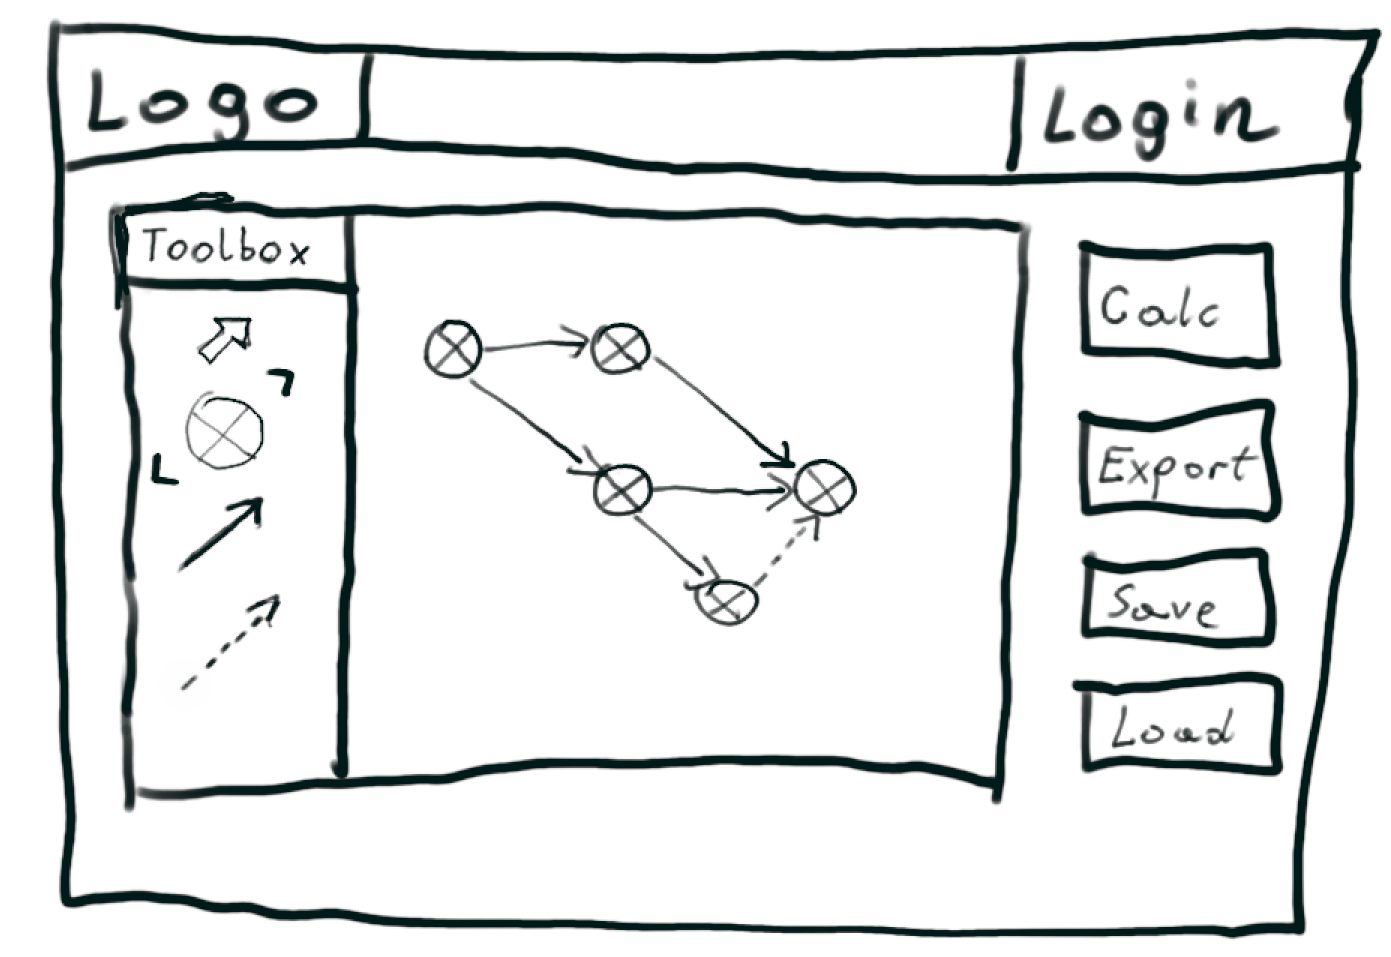
\includegraphics[width=0.9\linewidth]{main-window}
	\caption[Główne okno aplikacji]{Główne okno aplikacji}
	\label{fig:main-window}
\end{figure}
